Esse segue o mesmo arranjo do retificador a diodo. Pode-se ver na figura \ref{ccr} um simples circuito do retificador monofásico de meia onda a tiristor para uma carga resistiva. 

\begin{figure}[h]
\center
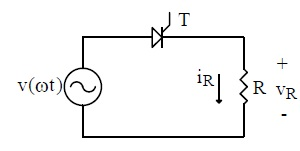
\includegraphics[scale=0.55]{imagens/circuito_carga_resistiva.jpg}
\caption{Circuito de um retificador a tiristor monofásico de meia onda com carga resistiva.}\label{ccr}
\caption*{Fonte: Eletônica de potência (2006)}
\end{figure}
  
Analisando as formas de onda na figura \ref{gcr} pode-se notar que até $\omega${t} = $\alpha$ a tensão na carga é nula, o que muda pela corrente de gatilho $i_{G}$. Assim, até o fim do semiciclo, a tensão de carga é igual à tensão da fonte. No semiciclo negativo, o tiristor encontra-se inversamente polarizado, i.e., não há tensão na carga.

\begin{figure}[h]
\center
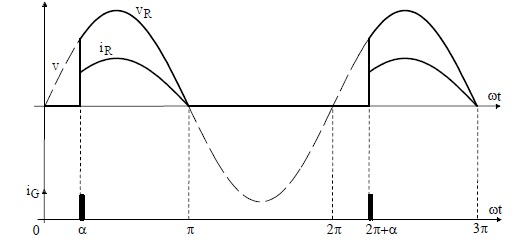
\includegraphics[scale=0.55]{imagens/grafico_carga_resistiva.jpg}
\caption{Formas de onda para retificador a tiristor monofásico de meia onda com carga resistiva.}\label{gcr}
\caption*{Fonte: Eletônica de potência (2006)}
\end{figure}

Portanto a tensão da fonte é calculada conforme a seguinte equação:
Assim, sendo $v(\omega t)=\sqrt{2}V_o\sin(\omega t)$ a tensão de alimentação, a tensão média na carga é
\begin{align*}
    V_{L,med} &= \frac{1}{2\pi}\int_\alpha^{\pi}\sqrt{2}V_o\sin(\omega t)d(\omega t) \\
&= \frac{\sqrt{2}V_o}{2\pi}[-cos(\omega t)]_\alpha^{\pi} \\
&\approx 0,225 V_o[1+\cos\alpha]
,\end{align*}
ou seja, a tensão média na carga é uma função do ângulo $\alpha$ de disparo do tiristor.

Dessa forma, a corrente média na carga é
\begin{align*}
    I_{L,med} &= \frac{V_{L,med}}{R} \\
    &\approx \frac{0,225 V_o}{R}(1+\cos\alpha)
.\end{align*}

A corrente eficaz na carga é
\begin{align*}
    I_{L,ef}&=\sqrt{\frac{1}{2\pi}\int_{\alpha}^{\pi}(\frac{\sqrt{2}V_o}{R})^{2}\sin^{2}(\omega t)d(\omega t)} \\
&=\sqrt{\frac{2V_o^{2}}{2\pi R^{2}}\int_{\alpha}^{\pi}\sin^2(\omega t)d(\omega t)} \\
&=\frac{V_o}{R}\sqrt{\frac{1}{\pi}\int_{\alpha}^{\pi}\sin^2(\omega t)d(\omega t)} \\
&=\frac{V_o}{R}\sqrt{\frac{1}{2}-\frac{\alpha}{2\pi}+\frac{\sin^2\alpha}{4\pi}}
.\end{align*}
A partir dela, pode-se determinar a potência por
\begin{align*}
    P_{R}&=RI_{L,ef}^{2} \\
	 &=\frac{V_{o}^{2}}{R}\left(   \frac{1}{2}-\frac{\alpha}{2\pi}+\frac{\sin^2\alpha}{4\pi}\right)
.\end{align*}

Caso a carga tenha um componente indutivo como no circuito da figura \ref{cti}, a característica indutiva gera um atraso na corrente, o que acarreta, tal qual no retificador a diodo, em um ângulo de bloqueio do diodo $\beta > \pi$, além do já estudado ângulo $\alpha$ para entrada em condução. As formas de onda da tensão e corrente na carga são ilustradas pela figura \ref{gti}.

\begin{figure}[h]
\center
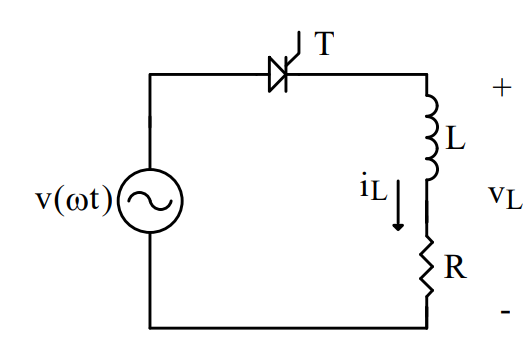
\includegraphics[scale=0.55]{imagens/circuito_tiristor_indutor.png}
\caption{Circuito de um retificador monofásico de meia onda a tiristor com carga indutiva.}\label{cti}
\caption*{Fonte: Eslaides aula 7 retificador a tiristor - Denizar Martins}
\end{figure}

\begin{figure}[h]
\center
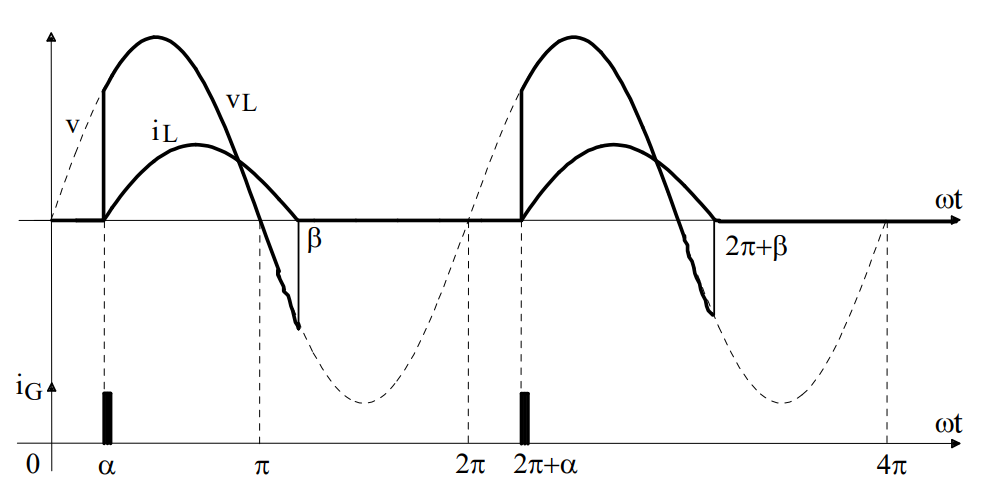
\includegraphics[scale=0.55]{imagens/grafico_tiristor_indutor.png}
\caption{Formas de onda de um retificador monofásico de meia onda a tiristor com carga indutiva.}\label{gti}
\caption*{Fonte: Eslaides aula 7 retificador a tiristor - Denizar Martins}
\end{figure}

Mais uma vez, sabe-se que, a partir do ângulo $\alpha$, a tensão na malha pode ser expressa através da corrente $i_L$ na carga, ou seja, \[
0 = Ri_{L}(wt) + L\frac{di_{L}(wt)}{dt} -v(wt)
,\] logo, \[
i_{L}(\omega{t}) = {\frac{\sqrt{2}V_o}{\sqrt{R^2 + X^2}}\sin{\left(\omega{t}-\phi\right)}e^{-t/\tau}}
,\] onde $\phi = \arctan{\frac{X}{R}}$, $ {X} = \omega{L} $ e $\tau = \frac{L}{R}$.

Podemos entender a corrente como a soma de dois componentes $i_L = i_1 + i_2$, sendo esses 
\begin{align*}
    i_{1}(\omega{t}) &= {\frac{\sqrt{2}V_o}{\sqrt{R^2 + X^2}}\sin{\left(\omega{t}-\phi\right)}} \\
    i_{2}(\omega{t}) &= {\frac{-\sqrt{2}V_o}{\sqrt{R^2 + X^2}}\sin{\left(\alpha-\phi\right)}e^{\frac{-t}{\tau}}}
.\end{align*}
Esses componentes representam, respectivamente, a corrente que circula em regime permanente e a corrente do transitório.

A tensão média na carga é
\begin{align*}
    V_{L,med} &= \frac{1}{2\pi}\int_\alpha^{\beta}\sqrt{2}V_o\sin(\omega t)d(\omega t) \\
&\approx 0,225 V_o[\cos\alpha - \cos\beta]
.\end{align*}
Fixando $V_{o}$ e $\alpha$, vemos que a tensão média na carga é função do ângulo $\beta$ que é uma função da constante de tempo da carga. Além disso, verificamos o resultado pela validade para a carga resistiva, em que $\beta = 1$, uma vez que as equações coincidem com as já discutidas.

A partir da tensão média, determinamos a corrente média na carga 
\begin{align*}
    I_{L,med} &= \frac{V_{L,med}}{R} \\
    &\approx \frac{0,225 V_o}{R}(\cos\alpha - \cos\beta)
.\end{align*}

O ângulo $\beta$ que controla o bloqueio do diodo pode ser determinado a partir de
\begin{align*}
    0 &= \frac{\sqrt{2}V_o}{\sqrt{R^2 + X^2}} \left[  \sin{\left(\beta-\phi\right)} -\sin{\left(\alpha-\phi\right)}e^{-\frac{\omega{R}}{\omega{L}}\left(  t -\frac{\alpha}{\omega}\right)} \right]  \\
    \implies 0 &= \sin(\beta - \phi) - \sin(\alpha - \phi)e^{\frac{R}{\omega{L}}(\beta - \alpha)}
,\end{align*}
que pode ser solucionada numericamente.

Com isso, determinamos a corrente eficaz na carga
\begin{align*}
    I_{L,ef}&=\sqrt{\frac{1}{2\pi}\int_{\alpha}^{\beta}i_{L}(\omega{t})^{2}d(\omega{t})} \\
&=\sqrt{\frac{1}{2\pi}\int_{\alpha}^{\beta}\left[\frac{\sqrt{2}V_{o}}{\sqrt{R^2 + X^2}}\left(  \sin(\omega{t}- \phi) - \sin(\alpha - \phi)e^{-\frac{R}{\omega{L}}(\omega{t}-\alpha)}\right)  ^{2}  \right] d(\omega{t})}
.\end{align*}

Para mitigar o problema da tensão negativa sobre a carga, pode-se adicionar ao circuito um diodo roda livre, resultando no circuito visível na figura \ref{cdc1}. Assim, também ilustrado na figura, o diodo permite a passagem da corrente induzida pelo indutor.

\begin{figure}[h]
\center
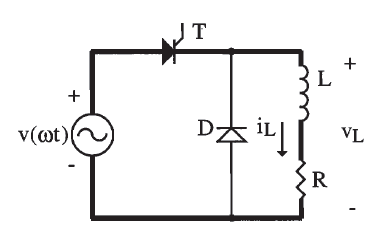
\includegraphics[width=0.45\textwidth]{imagens/circuito_diodo_circulacao1.png}
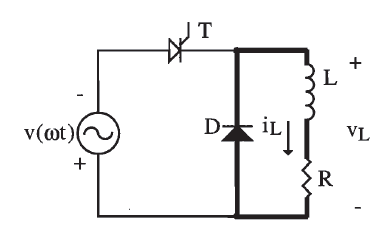
\includegraphics[width=0.45\textwidth]{imagens/circuito_diodo_circulacao2.png}
\caption{Circuito do retificador monofásico de meia onda a tiristor com diodo roda livre.}\label{cdc1}
\caption*{Fonte: Eletrônica de potência (2006)}
\end{figure}


A tensão e a corrente na carga estão representadas na figura \ref{gdc}. Vemos que a corrente na carga atinge seu valor máximo quando $\omega{t} = \omega{t}_{m}$, quando
\begin{align*}
    \frac{di_{L}(\omega{t})}{d(\omega{t})}&=0   \\
v_{1}(\omega{t})&=0
.\end{align*}

\begin{figure}[h]
\center
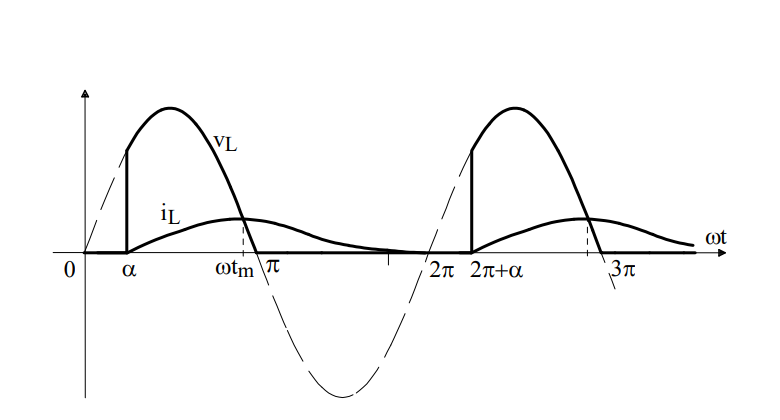
\includegraphics[scale=0.55]{imagens/formas_de_onda.png}
\caption{Tensão e corrente na carga do retificador monofásico de meia onda a tiristor com diodo de circulação.}\label{gdc}
\caption*{Fonte: Eletrônica de potência (2006)}
\end{figure}

A tensão média na carga é 
\begin{align*}
    V_{L,med} &= \frac{1}{2\pi}\int_{\alpha}^{\pi}\sqrt{2}V_{o}\sin(\omega{t}d(\omega{t}) \\
&= \frac{\sqrt{2}V_{o}}{2\pi}[-\cos(\omega{t})]_{\alpha}^{\pi} \\
&\approx 0,225V_{o}(1+\cos\alpha)
.\end{align*}
Veja que a tensão média não mais depende do ângulo $\beta$ e nem, portanto, da corrente de carga.

É evidente pela ilustração do seu comportamento que a corrente na carga se comporta de forma distinta em cada semiciclo da alimentação.

No semiciclo positivo, após $\alpha$, temos \[
i_{L1}(\omega{t}) = \frac{\sqrt{2}V_{o}}{\sqrt{R^2+X^2}}[\sin(\omega{t}-\phi)-\sin(\alpha-\phi)e^\frac{-t'}{\tau}]
,\] em que $t'=t-\frac{\alpha}{\omega}$.

No semiciclo negativo, até $\theta=\pi+5\omega \tau$,\[
i_{L1}(\omega(t)) = I_{1}e{^\frac{-t}{\tau}}
,\] onde $t''=t-\frac{\pi}{\omega}$.

Assim, \[
I_{1} = \frac{\sqrt{2}V_{o}}{\sqrt{R^2+X^2}}[\sin(\omega{t}-\phi)-\sin(\alpha-\phi)e^\frac{(\pi-\alpha)}{\omega\tau}]
,\] que nos permite refinar a nossa fórmula para a corrente de carga como \[
i_{L2}(\omega{t}) = \frac{\sqrt{2}V_{o}}{\sqrt{R^2+X^2}}[\sin(\omega{t}-\phi)-\sin(\alpha-\phi)e^\frac{(\pi-\alpha)}{\omega\tau}]e^\frac{(t-\pi/\omega)}{\tau}
.\] 

